\documentclass{article}

% Language setting
% Replace `english' with e.g. `spanish' to change the document language
\usepackage[english]{babel}

% Set page size and margins
% Replace `letterpaper' with`a4paper' for UK/EU standard size
\usepackage[letterpaper,top=2cm,bottom=2cm,left=3cm,right=3cm,marginparwidth=1.75cm]{geometry}

% Useful packages
\usepackage{amsmath}
\usepackage{graphicx}
\usepackage[colorlinks=true, allcolors=blue]{hyperref}

\title{Projet MOGPL}
\author{Antoine TOULLALAN Noureddine YAKHOU}

\begin{document}
\maketitle

\section*{Question 1 :}

\subsection*{Assertion 1} Un sous-chemin préfixe d’un chemin d’arrivée au plus tôt peut ne pas être un chemin d’arrivée au plus tôt.
\\Si on prend le chemin de a à d $\lbrace$ a-(4)$\mapsto$c-(5)$\mapsto$d$\rbrace$ qui est un chemin d’arrivée au plus tôt le sous chemin de  a à c $\lbrace$ a-(4)$\mapsto$c $\rbrace$ n’est pas un chemin d’arrivée au plus tôt car pour aller du sommet  a au sommet c le chemin d’arrivée au plus tôt est le chemin $\lbrace$ a-(1)$\mapsto$b-(2)$\mapsto$c $\rbrace$ vue que celui -ci nous permet d’arriver à c le jour 3 et que le chemin direct nous permet d’arriver le  jour 5.
\\
\begin{center}
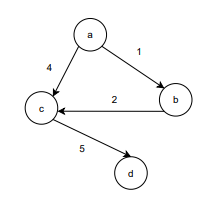
\includegraphics[width=0.4\textwidth]{qp.png}
\end{center}
\\
\subsection*{Assertion 2} Un sous-chemin postfixe  d’un chemin de départ au plus tard peut ne pas être un chemin de départ au plus tard.
\\Si on prend le chemin de départ au plus tard de a à c qui est $\lbrace$ a-(2) $  \mapsto$ b-(3)$\mapsto$c $\rbrace$ son sous chemin de b à c n’est pas un chemin de départ au plus tard car pour aller du sommet b au sommet c le chemin de départ au plus tard est$\lbrace$ b-(4) $\mapsto$c $\rbrace$
\\
\begin{center}
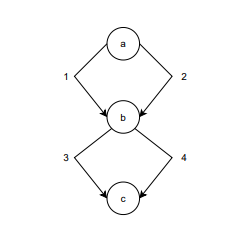
\includegraphics[width=0.4\textwidth]{qd.png}
\end{center}



\subsection*{Assertion 3 } Un sous chemin d’un chemin le plus rapide peut ne pas être le chemin le plus rapide.
\\Si on prend le chemin le plus rapide dans notre cas qui est $\lbrace$ a-(3)-d-(5)-e $\rbrace$ son sous chemin pour aller de a à d n’est pas le chemin le plus rapide car pour aller de a à d le chemin$\lbrace$ a-(2)$\mapsto$b-(3)$\mapsto$d $\rbrace$ est le chemin de plus rapide vue qu’il nous permet d’arriver à d le jour 4 tant dis que notre sous chemin de départ nous permet d’arriver à d le jour 6.
\\
\begin{center}
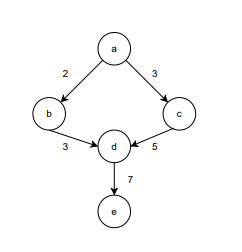
\includegraphics[width=0.4\textwidth]{qt.png}
\end{center}

\\
\subsection*{Assertion 4 }: un sous chemin d’un plus court chemin peut ne pas être un plus court chemin.
\\Dans notre cas le chemin le plus court pour aller de a à l est $\lbrace$a-(1)$\mapsto$b-(2)$\mapsto$c-(3)$\mapsto$d $\rbrace$ vue que le chemin $\lbrace$a-(4)$\mapsto$c-(3)$\mapsto$d $\rbrace$ n’est pas possible ,le sous chemin de a à c n’est pas le plus court chemin vue qu’il s’étend sur  2 arc et que le chemin $\lbrace$ a-(4)$\mapsto$c $\rbrace$ prend seulement un arc ce qui fait que ce dernier est le plus court chemin.
\\
\begin{center}
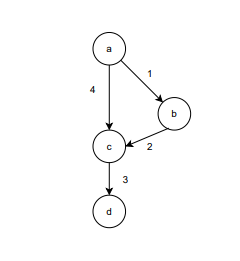
\includegraphics[width=0.4\textwidth]{qq.png}
\end{center}
\section*{Question 2 :}

\subsection*{Calcul du chemin de type I}
Pour calculer le chemin d'arrivée au plus tôt P dans G tel que $ P \in P(x, y, [td, tf]) $, on construit  \~G  = (\~V,\~E).
Dans \~G, on prend x' = (x,tmin) le sommet de départ avec tmin = min(t \| $ (x,t) \in $ \~E, $ t \geq td $ ) et y' = (y,tmax) le sommet d'arrivée avec tmax = max(t \| $ (y,t) \in $ \~E, $ t \leq tf $).\\
On modifie \~G: pour tous les sommets s \textbf{sauf y}, pour chaque arcs (s, $ t_{i} $) → (s, $ t_{i+1} $), on met un poids égale à $ t_{i+1} - t_{i} $ à cet arc.C'est à dire qu'on ajoute les temps d'attente pour chaque sommet de G.\\

On calcule ensuite avec l'algorithme de Djikstra le chemin de moindre coût de x' à y'.
On a ainsi un chemin P' dans \~G (v0,v1,v2,...,vn). Pour avoir un chemin P dans G, on prend les sommets appartenant à G qui sont visités dans P' dans le même ordre. Par exemple, si dans l'exemple de graphe \~G de l'énoncé, on a le chemin de a à f avec notre algorithme: P'=((a,1),(a,2),(b,3),(b,5),(f,6),(f,7)), \\le chemin associé dans P sera P= (a,b,f) avec l'arête de a-b =(a,b,2,1) et l'arête b-f =(b,f,5,1) avec une arrivée dans f à t=6 qui est bien l'arrivée la plus tôt.\\

On a ainsi un chemin dans P qui est le chemin d'arrivée au plus tôt car dans \~G, chaque arête est pondéré par le temps d'attente/trajet depuis sauf pour les arêtes entre les sommets y où le poids est 0. Le chemin de moindre cout dans \~G est donc le chemin qui "arrive" après le moins de temps d'attente/trajet possible à un sommet (y,t), càd qui permet d'avoir le moins de temps entre le sommet de départ et le sommet d'arrivée.\\
On a donc bien un chemin qui est celui de l'arrivée la plus tôt de x à y.\\

Exemple du graphe G modifié dans l'annexe.
\subsection*{Calcul du chemin de type II}
Pour le calcul du chemin de départ P le plus tard dans G tel que $ P \in P(x, y, [td, tf]) $, on construit  \~G  = (\~V,\~E). Comme dans le calcul du chemin I, dans \~G, on prend x' = (x,tmin) le sommet de départ avec tmin = min(t \| $ (x,t) \in $ \~E, $ t \geq td $ ) et y' = (y,tmax) le sommet d'arrivée avec tmax = max(t \| $ (y,t) \in $ \~E, $ t \leq tf $).\\
On modifie \~G: pour tous les sommets s \textbf{sauf x}, pour chaque arcs (s, $ t_{i} $) → (s, $ t_{i+1} $), on met un poids égale à $ t_{i+1} - t_{i} $ à cet arc.\\

On calcule ensuite avec l'algorithme de Djikstra le chemin de moindre coût de x' à y'. On a donc un chemin P' dans \~G.

De la même manière que dans le calcul du chemin I on passe d'un chemin P' dans \~G à un chemin P dans G.

P est le chemin de départ le plus tard car dans \~G, chaque arête est pondéré par le temps d'attente/trajet depuis sauf pour les arêtes entre les sommets x où le poids est 0. Le chemin de moindre coût de x' à y' dans \~G est donc le chemin qui "part" après le plus de temps d'attente possible d'un sommet (x,t) (x est le sommet de départ) car le chemin emprunte alors des arêtes de coût nuls, càd dont le coût est inférieurs aux autres arêtes qui "part" après moins de temps d'un sommet (x,t), c'est donc le sous-chemin que va emprunter le chemin de moindre cout.

On a donc bien un chemin qui est celui de départ le plus tard de x à y.\\
Exemple du graphe G modifié dans l'annexe.
\subsection*{Calcul du chemin de type III}
Pour le calcul du chemin le plus rapide P dans G tel que $ P \in P(x, y, [td, tf]) $, on construit  \~G  = (\~V,\~E). Comme dans le calcul du chemin I et II, dans \~G, on prend x' = (x,tmin) le sommet de départ avec tmin = min(t \| $ (x,t) \in $ \~E, $ t \geq td $ ) et y' = (y,tmax) le sommet d'arrivée avec tmax = max(t \| $ (y,t) \in $ \~E, $ t \leq tf $).\\
On modifie \~G: pour tous les sommets s \textbf{sauf x et y}, pour chaque arcs (s, $ t_{i} $) → (s, $ t_{i+1} $), on met un poids égale à $ t_{i+1} - t_{i} $ à cet arc.\\

On calcule ensuite avec l'algorithme de Djikstra le chemin de moindre coût de x' à y'. On a donc un chemin P' dans \~G.

De la même manière que dans le calcul du chemin I on passe d'un chemin P' dans \~G à un chemin P dans G.\\

P est le chemin le plus rapide car les arêtes dans \~G connectant les sommets (x,t) entre eux sont nulles, idem pour les les arêtes connectant les sommet (y,t).Ainsi, dans le chemin de moindre coût on maximise les temps d'"attente" dans les sommets de départ et d'arrivée, donc on minimise les temps de trajet/attente entre les sommets de départ et les sommets d'arrivée dans P'. On a donc un chemin avec un temps de trajet/attente minimal dans P. \\

On a donc bien un chemin qui est le plus rapide de x à y.\\
Exemple du graphe G modifié dans l'annexe.
\subsection*{Calcul du chemin de type IV}
Pour le calcul du chemin le plus court P dans G tel que $ P \in P(x, y, [td, tf]) $, on construit  \~G  = (\~V,\~E). Contrairement aux parties précédentes, on ne modifie pas \~G.\\
On prend x' = (x,tmin) le sommet de départ avec tmin = min(t \| $ (x,t) \in $ \~E, $ t \geq td $ ) et y' = (y,tmax) le sommet d'arrivée avec tmax = max(t \| $ (y,t) \in $ \~E, $ t \leq tf $).\\

On calcule ensuite avec l'algorithme de Djikstra le chemin de moindre coût de x' à y'. On a donc un chemin P' dans \~G.De la même manière que dans le calcul du chemin I on passe d'un chemin P' dans \~G à un chemin P dans G.\\

Ce chemin P est le plus court dans G car comme P' est de moindre cout dans \~G, on change d'aéroport le moins souvent possible.\\

On a donc bien un chemin P qui est le plus court de x à y.\\
Exemple du graphe G modifié dans l'annexe.
\section*{Question 3 :}
Pour les 4 chemins, on calcule avec un algorithme de Djikstra le chemin de moindre coût sur un graphe qui a le même nombre de sommets et d'arêtes. Donc les 4 algorithmes ont la même complexité.\\

Soit le sommet G avec n sommets et m arêtes, on suppose qu'on calcule les chemins I,II,III,IV dans P(x,y,[td,tf]) et que $ td \geq tf $.On a pour chaque sommet de G, au plus tf-td sommets associés dans \tild G (au plus tf-td temps sont associé à chaque sommet), et donc au plus tf-td-1 arêtes supplémentaires car ces "nouveaux" sommets sont connectés entre eux dans \tild G.\\

Donc dans \tild G, soit n' le nombre de sommet et m' le nombre d'arêtes, on a $ n' \leq n*(tf-td) $ et $ m' \leq m+(tf-td)*n $. Or lors des calculs des chemins I,II,III,IV, on applique un algorithme de Djikstra, donc la complexité des algorithmes est: O($ n'^2 $) donc O($ (tf-td)^{2}*n^{2} $).\\

Donc la complexité des algorithmes des chemins I,II,II,IV est O($ (tf-td)^{2}*n^{2} $).
\section*{Question 5 :}

Supposons qu'on ait un multigraphe G sans cycle. Pour calculer le plus court chemin du chemin x à y, on calcule le graphe \tild G associé avec n sommets (qu'on note s1,s2...sn) et m arêtes (qu'on note a1,a2..am).
A partir de \tild G, on crée le programme linéaire P avec m+1 contrainte et n variables:\\

On ajoute une borne supérieure aux variables de P, car dans le cas où un sommet n'est pas accessible depuis le sommet de départ, la variable associée à ce sommet ne sera pas bornée (avec une borne supérieure). Il faut que cette borne soit supérieure aux variables des sommets qui ont comme voisin le sommet d'arrivée. Donc ,si le calcul du chemin IV se fait dans P(x,y,[td,tf], on prend comme borne supérieure tf+1.\\

Soit s le sommet (x,t) dans \tild G avec t=min \{t \| (x,t)$ \in $ \tild V\}\\

Max s1+s2+...+sn\\

s=0\\ ou s$ \leq $0
Pour chaque arête ai=(si,sj,val), on crée la contrainte\\
sj-si$ \leq $ val\\

s1,s2,...,sn$ \geq $ 0

La résolution de P donne une valeur à chaque sommet car chaque variable représente un sommet dans \tild G. Pour chaque sommet si, on a donc la valeur vi qui est la longueur du plus court chemin de x à si.\\
Pour connaitre le plus court chemin de x à y, on se place au sommet y et on prend ,parmi les sommets qui ont comme voisins y, celui qui a la valeur associée la plus petite, à partir de ce sommet s1 on prend, parmi les sommets qui ont comme voisins s1, celui qui a la valeur associée la plus petite,... on itère jusqu'a être au noeud x. On a ainsi le chemin le plus court de x à y.\\

En annexe, on montre le programme linéaire pour le multigraphe G de l'énoncé.

\section*{Question 6 :}
On observe les temps de calcul de la méthode utilisant gurobi en fonction du nombre de sommets du graphe, et du nombre d'arêtes.\\Pour influer sur le nombre d'arêtes du multigraphe, on modifie la probabilité p de jonction de 2 sommets par 1,2 ou 3 arêtes (de manière aléatoire).\\ 

Pour chacun de ces 2 paramètres, on en fait varier un en fixant l'autre, on a ainsi les graphes suivants en échelles logarithmique:\\
\newpage
\begin{center}
\textbf{Log Nombre de sommets en fonction du log de temps de calcul\\}
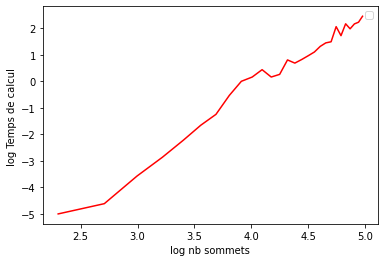
\includegraphics[width=0.7\textwidth]{dsommets.png}\\
On voit qu'on a une forme de droite qui a un coefficient directeur d'environ 3 (2.7). On en déduit que le temps de calcul de notre méthode évolue de manière polynomiale en fonction du nombre de sommets avec un coefficient de 3\\.

\textbf{Log de la probabilité de jonction de sommets en fonction du log de temps de calcul\\}
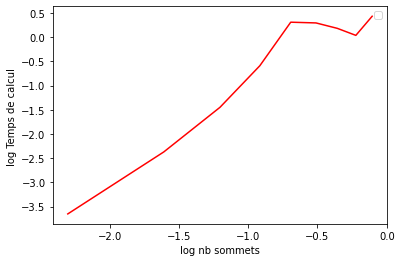
\includegraphics[width=0.7\textwidth]{daretes.png}\\
On a ici aussi une forme de droite avec un coefficient directeur d'environ 2. On en déduit que le temps de calcul évolue de manière polynomiale en fonction du nombre d'arêtes avec un coefficient de 2.\\
\end{center}
On peut en déduire que la complexité de notre algorithme utilisant gurobi est $ O(n^{3}*p^{2}) $ pour un graphe avec n sommets et m arêtes et un intervalle de temps [td,tf].

\newpage
\section*{ANNEXE :}

On prend les graphes modifiés à partir du graphe G de l'énoncé.\\
On a départ=a, arrivée=f, et [td,tf]=[1,8].
\begin{center}
\subsection*{Chemin I}
\centering
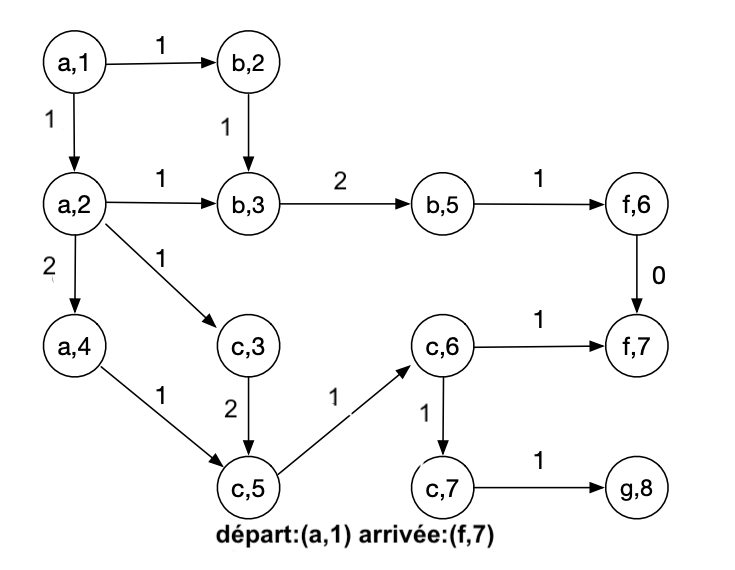
\includegraphics[width=0.5\textwidth]{chemin_I.png}
\subsection*{Chemin II}
\centering
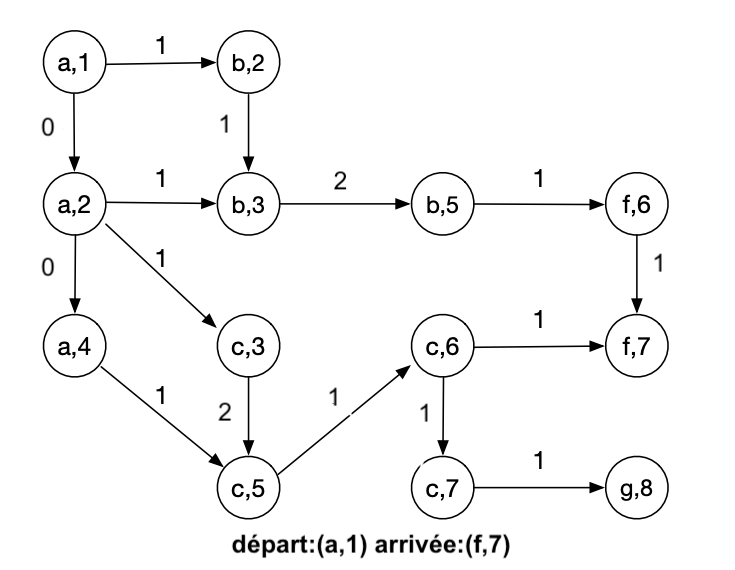
\includegraphics[width=0.5\textwidth]{chemin_II.png}
\subsection*{Chemin III}
\centering
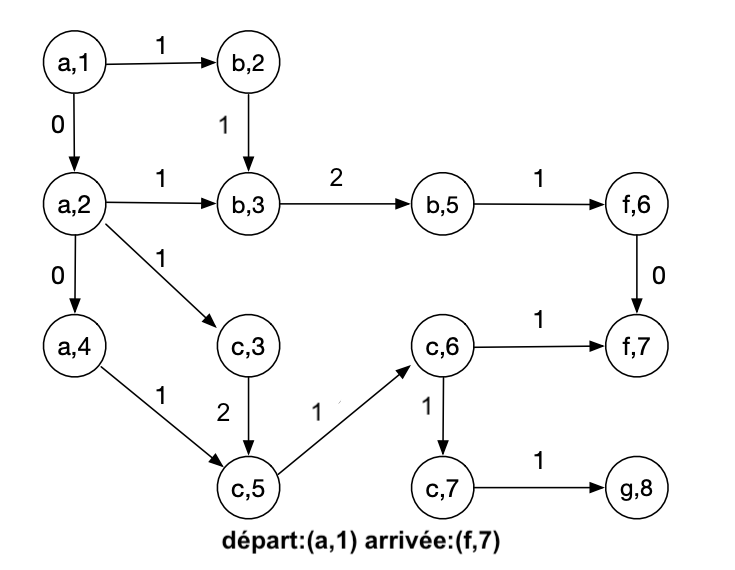
\includegraphics[width=0.5\textwidth]{chemin_III.png}
\subsection*{Chemin IV}
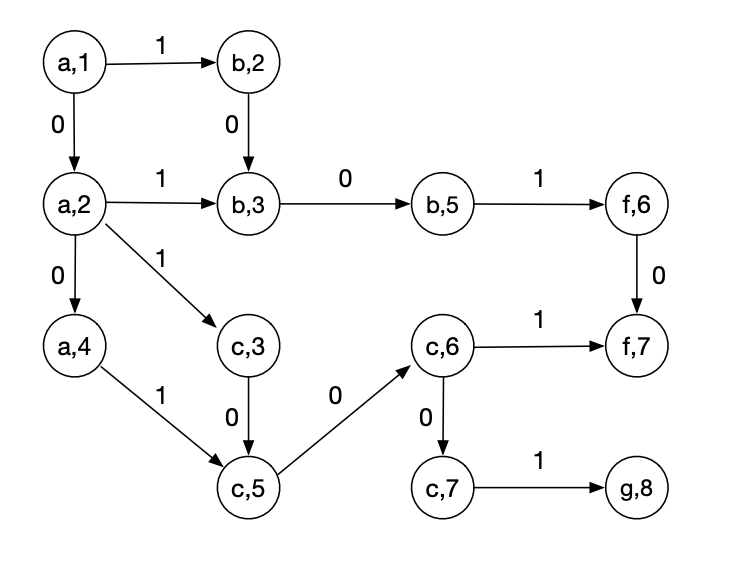
\includegraphics[width=0.5\textwidth]{chemin_IV.png}
\end{center}
\subsection*{Programme linéaire pour le chemin le plus court de a à f}

Max a1,a2,a4,b2,b3,b5,c3,c5,c6,c7,f6,f7,g8\\

a1$ \leq $0\\
b2-a1$ \leq $1\\
a2-a1$ \leq $0\\
a4-a2$ \leq $0\\
b3-a2$ \leq $1\\
b3-b2$ \leq $0\\
b5-b3$ \leq $0\\
c3-a2$ \leq $1\\
c5-a4$ \leq $1\\
c5-c3$ \leq $0\\
c6-c5$ \leq $0\\
c7-c6$ \leq $0\\
g8-c7$ \leq $1\\
f7-c6$ \leq $1\\
f6-b5$ \leq $1\\
f7-f6$ \leq $0\\

0$ \leq $ a1,a2,a4,b2,b3,b5,c3,c5,c§,c7,f6,f7,g8 $ \leq $ 9
\end{document}